%%%%%%%%%%%%%%%%%%%%%%%%%%%%%%%%%%%%%%%%%%%%%%%%%%%%%%%%%%%%%%%%%%%%%%%%%%%%%%%%
%2345678901234567890123456789012345678901234567890123456789012345678901234567890
%        1         2         3         4         5         6         7         8

\documentclass[a4paper, 10pt]{article}
\usepackage[a4paper, margin={2.5cm, 2.5cm}]{geometry}

% The following packages can be found on http:\\www.ctan.org
%\usepackage{epsfig} % for postscript graphics files
%\usepackage{mathptmx} % assumes new font selection scheme installed
%\usepackage{times} % assumes new font selection scheme installed
\usepackage{listings}
\usepackage{graphics}
\usepackage{amsmath}
\usepackage{amssymb}
\usepackage{acro}
\usepackage{enumitem}
\usepackage{graphicx}
\usepackage{wrapfig}
\usepackage{hyperref}
\usepackage{tabularx}
\usepackage{setspace}
\usepackage{comment}
\usepackage{mathrsfs}
\usepackage{tikz}
\usepackage{authblk}

\usepackage{color} %use color
\definecolor{mygreen}{rgb}{0,0.6,0}
\definecolor{mygray}{rgb}{0.5,0.5,0.5}
\definecolor{mymauve}{rgb}{0.58,0,0.82}
\definecolor{pagecolor}{rgb}{1,1,1}
\pagecolor{pagecolor}
%Customize a bit the look
\lstset{ %
backgroundcolor=\color{pagecolor}, % choose the background color; you must add \usepackage{color} or \usepackage{xcolor}
basicstyle=\footnotesize, % the size of the fonts that are used for the code
breakatwhitespace=false, % sets if automatic breaks should only happen at whitespace
breaklines=true, % sets automatic line breaking
captionpos=b, % sets the caption-position to bottom
commentstyle=\color{mygreen}, % comment style
deletekeywords={...}, % if you want to delete keywords from the given language
escapeinside={\%*}{*)}, % if you want to add LaTeX within your code
extendedchars=true, % lets you use non-ASCII characters; for 8-bits encodings only, does not work with UTF-8
frame=single, % adds a frame around the code
keepspaces=true, % keeps spaces in text, useful for keeping indentation of code (possibly needs columns=flexible)
keywordstyle=\color{blue}, % keyword style
% language=Octave, % the language of the code
morekeywords={*,...}, % if you want to add more keywords to the set
numbers=left, % where to put the line-numbers; possible values are (none, left, right)
numbersep=5pt, % how far the line-numbers are from the code
numberstyle=\tiny\color{mygray}, % the style that is used for the line-numbers
rulecolor=\color{black}, % if not set, the frame-color may be changed on line-breaks within not-black text (e.g. comments (green here))
showspaces=false, % show spaces everywhere adding particular underscores; it overrides 'showstringspaces'
showstringspaces=false, % underline spaces within strings only
showtabs=false, % show tabs within strings adding particular underscores
stepnumber=1, % the step between two line-numbers. If it's 1, each line will be numbered
stringstyle=\color{mymauve}, % string literal style
tabsize=2, % sets default tabsize to 2 spaces
title=\lstname % show the filename of files included with \lstinputlisting; also try caption instead of title
}
%END of listing package%
 
\definecolor{darkgray}{rgb}{.4,.4,.4}
\definecolor{purple}{rgb}{0.65, 0.12, 0.82}
 

%define Javascript language
\lstdefinelanguage{JavaScript}{
keywords={typeof, new, true, false, catch, function, return, null, catch, switch, var, if, in, while, do, else, case, break},
keywordstyle=\color{blue}\bfseries,
ndkeywords={class, export, boolean, throw, implements, import, this},
ndkeywordstyle=\color{darkgray}\bfseries,
identifierstyle=\color{black},
sensitive=false,
comment=[l]{//},
morecomment=[s]{/*}{*/},
commentstyle=\color{purple}\ttfamily,
stringstyle=\color{red}\ttfamily,
morestring=[b]',
morestring=[b]"
}
 
\lstset{
language=JavaScript,
extendedchars=true,
basicstyle=\footnotesize\ttfamily,
showstringspaces=false,
showspaces=false,
numbers=left,
numberstyle=\footnotesize,
numbersep=9pt,
tabsize=2,
breaklines=true,
showtabs=false,
captionpos=b
}
%---------------------------------------------------
%----- Hyper Setup
%---------------------------------------------------
\hypersetup{
	pdftitle={Centrifuge:  Protocol for private by design transactions on a decentralized network}, 
    pdfauthor={Lucas Vogelsang,Manuel Polzhofer, Philip Stehlik,Miguel Hervas Lazaro}, 
    pdfsubject={Protocol Paper, Centrifuge}, % please, select the type of this document
    pdfstartview={FitH},    % fits the width of the page to the windowhttps://www.overleaf.com/project/5c35d0fa8c97d86e2adb91c2
    pdfnewwindow=true, 		% links in new window
    colorlinks=true,  		% false: boxed links; true: colored links
    linkcolor=orange,          % color of internal links
    citecolor=orange,        % color of links to bibliography
    filecolor=magenta,      % color of file links
    urlcolor=black           % color of external links
}
% 


\makeatletter
\newcommand*{\xleftrightarrow}[2]{\mathrel{
  \settowidth{\@tempdima}{$\scriptstyle#1$}
  \settowidth{\@tempdimb}{$\scriptstyle#2$}
  \ifdim\@tempdimb>\@tempdima \@tempdima=\@tempdimb\fi
  \mathop{\vcenter{
    \offinterlineskip\ialign{\hbox to\dimexpr\@tempdima+1em{##}\cr
    \rightarrowfill\cr\noalign{\kern.5ex}
    \leftarrowfill\cr}}}\limits^{\!#1}_{\!#2}}}


%---------------------------------------------------
%----- Version
%---------------------------------------------------
\def\ProtocolPaperVersionNumber{unknown revision}
\IfFileExists{Options.tex}{\input{Options.tex}}

%---------------------------------------------------
%----- Helper Commands
%---------------------------------------------------
\newcommand{\codesection}[1]{\doublespacing{\hspace{\parindent}\texttt{#1}}}
\newcommand{\sbline}{\\[.5\normalbaselineskip]}% small blank line 
\newcommand{\ethleftarrow}{\ensuremath{\xleftarrow[]{\text{ETH}}}}


\title{\LARGE \bf
Centrifuge: Protocol for private by design transactions on a decentralized network
}
\date{\ProtocolPaperVersionNumber}
\author{Lucas Vogelsang\thanks{Lucas Vogelsang, {\tt\small l@lucasvo.com}} \hspace{0.1cm} Manuel Polzhofer\thanks{Manuel Polzhofer, {\tt\small manuel@centrifuge.io}}  \hspace{0.1cm} Philip Stehlik\thanks{Philip Stehlik, {\tt\small philip@centrifuge.io}} \hspace{0.1cm} Vimukthi Wickramasinghe\thanks{Vimukthi Wickramasinghe, {\tt\small vimukthi@centrifuge.io}} 
\newline Miguel Hervas Lazaro\thanks{Miguel Hervas Lazaro, {\tt\small miguel@centrifuge.io}}}


%%%%%%%%%%%%%%%%%%%%%%%%%%%%%%%%%%%%%%%%%%%%%%%%%%%%%%%%%%%%%%%%%%%%%%%%%%%%%%%%
\acsetup{first-style=short}

\begin{document}

\maketitle
\thispagestyle{empty}
\pagestyle{empty}

%---------------------------------------------------
%----- Content
%---------------------------------------------------
\input{abstract}
\input{1_introduction}
\input{2_high_level}
\input{3a_document_fields}
%---------------------------------------------------
%----- Version History
%---------------------------------------------------
\subsubsection{Version History}\label{sec:version_history}
The version history $H$ is a set of documents. An update of an existing document in the Centrifuge protocol happens by creating a new version and linking this new version to the previously existing version. 
We define the set of all documents as $D$:
\begin{equation}
d \in D
\end{equation}
Every node keeps a history of all versions of a document in which they are listed as a collaborator.
\begin{equation}
H = (d_{[0]},...,d_{[n]})
\end{equation}
\newline
In the initial version of a document $d_0$, the current version and the identifier will be equal.
\begin{equation}
d_{[0]{\texttt{id}}} = d_{[0]\texttt{current}}
\end{equation}
\newline
The fields for the previous document root hash $D_{\texttt{prev-root}}$ and for the $D_{\texttt{prev}}$ id will be empty in the initial version.
\begin{eqnarray}
d_{[0]{\texttt{prev-root}}}& = & \emptyset \\
d_{[0]{\texttt{prev}}} & = & \emptyset
\end{eqnarray}
\newline
For all other documents $D$ in a version history $H$, the following conditions must be true:
\newline
\newline
Every document in a version history $H$ must have the same identifier.
\begin{equation}
\{d_{[i]} \in H \mid \forall d_{[j]} \in H :d_{[i]\texttt{id}} = d_{[j]\texttt{id}} \}
\end{equation}
\newline
The current version field of a document must be equal to the next version field of the previous document.
\begin{equation}
d_{[i]\texttt{current}} = d_{[i-1]\texttt{next}} 
\end{equation}
\newline
The previous version field of a document must be equal to the current version field of the predecessor document.
\begin{equation}
d_{[i]\texttt{prev}} = d_{[i-1]\texttt{current}} 
\end{equation}
\newline
The previous root hash of a document must be equal to the document root hash of the predecessor document.
\begin{equation}
d_{[i]\texttt{prev-root}} = d_{[i-1]\texttt{doc-root}}
\end{equation}
\newline
The current pre-image of a document must be equal to the next pre image of the predecessor document.
\begin{equation}
d_{[i]\texttt{current-img}} = d_{[i-1]\texttt{next-img}}
\end{equation}
\newline
The history of the document can therefore be seen as a doubly linked list. Every document has the document hash $d_{\texttt{previous}}$ of the predecessor document and defines the $d_{\texttt{id}}$ of the next one.\\\\
A node which performs a document update defines the the next version identifier $d_{\texttt{next}}$.
\begin{equation}
d_{[i]\texttt{next-img}} = \texttt{RAND(32)}
\end{equation}
\begin{equation}
d_{[i]\texttt{next}} = \mathtt{blake2b}(d_{[i]\texttt{next-img}})
\end{equation}
\newline
The field $d_{\texttt{next-img}}$ is needed to prevent malicious anchoring of documents by non-collaborators. The value therefore must be kept secret from any non-collaborators. The function $\texttt{RAND(32)}$ is a cryptographically secure random function and returns a byte 32 array. The function $\mathtt{blake2b}$ denotes hash function blake2b-256. 

By referencing the previous root each state $d$, the history becomes an immutable attribute committed to in each version. To traverse the history $H$, one can follow the $d_{\mathtt{prev-root}}$ and $d_{\mathtt{prev}}$. To move forward in the list of history, $H$, one can go from $d_{\mathtt{next}}$ to $d_{\mathtt{current}}$.
\begin{figure}[thpb]
  \centering
  \includegraphics[width=16cm]{img/documents-history-v2.png}
  \caption{Doubly linked list of different versions of a document. Indicating the relationship between different document index fields. The document root $R_{\texttt{doc-root}}$ is stored in the anchor registry and not in the document itself.} 
  \label{fig:documents}
\end{figure}


%---------------------------------------------------
%----- Calculation of the Root Hashes
%---------------------------------------------------
\subsection{Calculation of the Root Hashes}
Every root hash of a document $R_{\texttt{doc-root}}$ is stored in the
\textit{AnchorRepository} smart contract. The document root hash is calculated from three different Merkle trees (see Fig. \ref{fig:root-hash}). 
\subsubsection{Merkle Tree of Fields}
A Merkle tree is a way to calculate a unique hash from a set of items. We formally define a Merkle tree function $\mathcal{M}$ to calculate a root hash $R \in \mathbb{B}_{32}$ of document fields $F$. The implementation of the Merkle tree function is introduced in Sec. \ref{sec:precise_proofs}.
 \begin{eqnarray}
 R & = &\mathcal{M}(F_{[0]},...,F_{[n]}) \\
 R & \in & \mathbb{B}_{32}
\end{eqnarray}
\newline
\subsubsection{Model Merkle tree}
As a first step, we calculate the Merkle tree of the schema fields $S$ and the core document fields $C$ of a document $d$.\\
As a second step, we flatten and combine all leaves from each tree.\\ 
Finally, we calculate the Model Merkle Root\\\\
\textbf{Model Root} The Merkle root of the flattened document schema and the core document data, formally $R_{{\texttt{model}}}$ 
\newline
\begin{equation}
    d_M = (d_S \cup d_C)
\end{equation}
\begin{equation}
    R_{{\texttt{model}}} = \mathcal{M}(d_M)
\end{equation}
\newline
 \subsubsection{Basic and ZK Model trees}
\textbf{Basic Model} The Merkle tree of the flattened document schema and the core document data, formally $R_{{\texttt{basic-model}}}$
\newline
\begin{equation}
    R_{{\texttt{basic-model}}} = \mathcal{M}(d_{MB})
\end{equation}
\newline
The Basic Model tree has the following properties:
\begin{itemize}  
\item Leaf Hashing function keccak-sha3 (add ref) of 256 bits
\item Node Hashing function blake2b (add ref) of 256 bits
\item Sorted Hashes
\end{itemize}
\newline
\textbf{ZK Model} The Merkle tree of the flattened document schema and the core document data ready for Zero Knowledge proving, formally $R_{{\texttt{zk-model}}}$
\newline
\begin{equation}
    R_{{\texttt{zk-model}}} = \mathcal{M}(d_{MZ})
\end{equation}
\newline
The ZK Model tree has the following properties:
\begin{itemize}  
\item Leaf Hashing function keccak-sha3 of 256 bits
\item Node Hashing function pedersen (add ref) of 256 bits
\item Ordered (Left-Right) Hashes
\item Fixed size of 20 levels
\end{itemize}
 \subsubsection{Signing Root}
The $R_{\texttt{signing}}$ is calculated from the blake2b-256 hash of the concatenated $R_\texttt{basic-model}$ and $R_{\texttt{zk-model}}$
\newline
\begin{equation}
R_{\texttt{signing}} = \texttt{blake2b}(R_\texttt{basic-model}\| R_{\texttt{zk-model}})
\end{equation}\\
We formally define a helper function for calculating the $R_{\texttt{signing}}$ 
\begin{eqnarray}
R_{\texttt{signing}}& =&\mathsf{calculateSigningRoot}(d) \\
\mathsf{calculateSigningRoot}(d)& =& \texttt{blake2b}(\mathcal{M}(d_{MB})\| \mathcal{M}(d_{MZ}))
\end{eqnarray}
 \subsubsection{Signatures Root}
 A Merkle root of the collaborator signature must be part of the document root hash $R_{\texttt{doc-root}}$. The signatures are relevant for the document consensus, explained in the following chapters. \\\\
\textbf{Signature Root} A signature root hash defines the Merkle root of all signatures $d_{\texttt{signatures}}$, formally $R_{\texttt{signatures}}$:
\newline
\begin{equation}
R_{\texttt{signatures}} = \mathcal{M}(d_{\texttt{signatures}})\\
\end{equation}
 \subsubsection{Document Root}
The final  document root hash $R_{\texttt{doc-root}}$ of the entire document $d$ is defined as the blake2b hash of the concatenated signing root hash $R_{\texttt{signing}}$ and signature root hash $R_{\texttt{signatures}}$ 
\newline
 \begin{equation}
R_{\texttt{doc-root}} =  \texttt{blake2b}(R_{\texttt{signing}}\|R_{\texttt{signatures}})
\end{equation}\\
A tree of the  $R_{\texttt{doc-root}}$ calculation. (see Fig. \ref{fig:root-hash})

%TODO (Manuel): Why sometimes R and D?

%All information related to the document is stored in a structured protobuf message called CoreDocument, \mathsf{CD}, along with a document-specific message, Data, \mathsf{D} such as an Invoice or PurchaseOrder. Both messages are serialized with precise proofs into \\mathsf{CD} 

\begin{figure}[thpb]
\centering
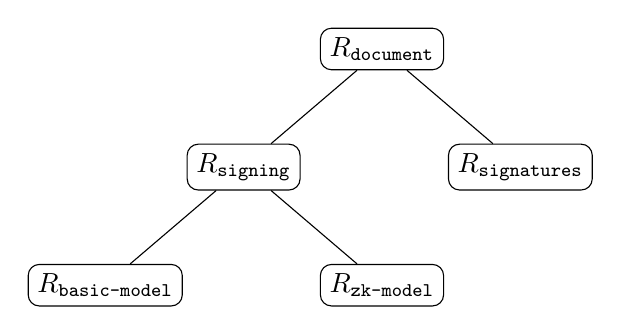
\begin{tikzpicture}[sibling distance=10em,
  every node/.style = {shape=rectangle, rounded corners,
    draw, align=center, %top color=white, bottom color=gray!20
    }]]
  \node {$R_{{\texttt{document}}}$}
    child { node {$R_{{\texttt{signing}}}$}  child { node {$R_{{\texttt{basic-model}}}$}  
    } child { node {$R_{{\texttt{zk-model}}}$} 
    } }
    child { node {$R_{{\texttt{signatures}}}$}};
\end{tikzpicture}
\caption{Calculation of the last layers of the document merkle tree. The leafs are the roots of merkle trees from the different document parts }\label{fig:root-hash}
\end{figure}
We can define a second help function called $\mathsf{calculateDocumentRoot}(d)$ for calculating the entire $R_{\texttt{doc-root}}$. 
\begin{eqnarray}
R_{\texttt{doc-root}}& =&\mathsf{calculateDocumentRoot}(d) \\
\mathsf{calculateDocumentRoot}(d)& = & \texttt{blake2b}( \mathsf{R_{\texttt{signing}}}\| \mathcal{M}_{\texttt{tree}}(d_S))
\end{eqnarray}
% describe how a document root hash is calculated
%---------------------------------------------------
%----- State Commitment
%---------------------------------------------------
\subsection{State commitment}

\subsubsection{Anchors}
An anchor is the root hash of a document $R_{\texttt{doc-root}}$ stored in an Ethereum smart contract called \textit{AnchorRepository}. 
\\\\
Every new document version $d'$ must commit its  document root hash $R_{\texttt{doc-root}}$ to the registry. A new document $d'$ is only valid and accepted if the $R_{\texttt{doc-root}}$ exists as an anchor in the registry.\\
%\textcolor{gray}{TODO: introduce blockheight}
\begin{eqnarray}
A &=& (A_{\texttt{anchor-id}}, A_{\texttt{anchor-root}}, A_{\texttt{anchor-blockheight}})\\
A_{\texttt{anchor-id}} & = & d_{\texttt{current}} \\
A_{\texttt{anchor-root}} & = & R_{\texttt{doc-root}} \\
A_{\texttt{anchor-blockheight}} & = & \texttt{block.number}
\end{eqnarray}
\\
The anchor id of a new document $d_{[i]{\texttt{current}}}$ is defined by the previous document $d_{[i-1]\texttt{next-img}}$. The same image is stored in the current 
document in $d_{[i]\texttt{current-img}}$. The hash of the $d_{[i]\texttt{current-img}}$ defines the current document identifier and the anchor id.
\begin{eqnarray}
d_{[i]\texttt{current}}& = & \mathtt{blake2b}(d_{[i-1]\texttt{next-img}})\\
A_{\texttt{anchor-id}}& = & d_{[i]\texttt{current}}
\end{eqnarray}
The \texttt{block.number} contains the Ethereum block number the transaction got mined and acts as a timestamp for the anchor.
\subsubsection{Verifying a document}
Any user can verify the correctness of the document by comparing the root hash to the committed hash on chain. We formally define a method called $\mathsf{getAnchor}$ which returns an anchor from the contract.
\begin{eqnarray}
A_{\texttt{anchor-current}} & \xleftarrow[]{\text{ETH}}& \mathsf{getAnchor}(d_{[i]{\texttt{current}}}) \\
A_{\texttt{anchor-next}} & \xleftarrow[]{\text{ETH}} & \mathsf{getAnchor}(d_{[i]{\texttt{next}}}) \\
\end{eqnarray}

\subsubsection{Latest Version}
Because in each document (state) update the next anchor id is already defined, anyone can verify that they have the latest version by checking the anchor registry. A document $d_{[i]}$ is the latest version if the following condition is true:
\begin{equation}
A_{\mathtt{anchor-current}} = R_{\mathtt{doc-root}} \quad \wedge \quad A_{\mathtt{anchor-next}} = 0
\end{equation}
If an anchor for $A_{\mathtt{anchor-next}}$ exists, the current document $d_{[i]}$ is not the latest version. It is not possible to overwrite an existing anchor id or invalid it. For committing an anchor the $d_{[i]\texttt{current-img}}$ is needed therefore only document collaborators could propose a next version.

\subsubsection{Pre-Commit}
A document is committed only after reaching consensus with the other collaborators on the document. Consensus is reached by getting a cryptographic signature from other parties by sending them the signing root. To deny the counter-party the free option of publishing its own state commitment upon receiving a request for signature, the node can first publish a pre-commit.
A pre-commit locks a commit to a specific document state for a given anchor id for a predetermined number of blocks. Only the \texttt{msg.sender} of the pre-commit is allowed to commit a corresponding anchor before the pre-commit has expired.

\begin{equation}\\
    \mathsf{preCommit}(d_{[i]\texttt{current}},R_{\texttt{signing}}) \xrightarrow[]{\text{ETH}} \mathsf{AnchorRepository}
    %TODO: leftover? M_{\texttt{proof}}(R_{\texttt{doc-root}})
\end{equation}\\
The pre-commit stores the provided signing root $R_{\texttt{signing}}$ on the smart contract. Only a $R_{\texttt{doc-root}}$ in the commit which includes the same $R_{\texttt{signing}}$ is accepted as a valid commit. 
It is not possible to provide a new preCommit $R_{\texttt{signing}}$ within the next  blocks for the given anchorId.\\
In the event that the user does not provide a commit within the lock time, the commit will be unlocked, and the \texttt{preCommit} method will be open to everyone again.

\subsubsection{Commit}
The anchor registry's \texttt{commit} method does not have any restrictions, except for the pre-commit flow as described above. If no valid pre-commit exists, anyone can commit an anchor to the registry. A commit of a new anchor is described by the following function. 
\begin{equation}\\
    \mathsf{commit}(d_{[i]\texttt{current-img}},R_{\texttt{doc-root}},P_{\texttt{sign-proof}}) \xrightarrow[]{\text{ETH}} \mathsf{AnchorRepository}
    %M_{\texttt{proof}}(R_{\texttt{doc-root}})
\end{equation}\\
\textbf{Next Pre-Image }\\
The commit method hashes $d_{[i−1]\texttt{next-img}}$ inside the smart contract to get the $A_{\texttt{anchor-id}}$. The $d_{[i−1]\texttt{next-img}}$ of the previous version is needed to commit the next version. It is not possible to use $d_{[i−1]\texttt{next}}$ (equal to $d_{[i]\texttt{current}}$) directly. In some cases, the field  $d_{\texttt{next}}$ is revealed to the outside world to prove the latest version of a document. (See \ref{sec:nft}). The anchor contract challenges the submitter to reveal the pre-image to avoid an attacker committing an malicious anchor for $d_{\texttt{next}}$. The field $d_{\texttt{next-img}}$ is never revealed to the outside world. \\
\\
\textbf{Signing Root Proof }\\
In case a pre-commit exists for the \texttt{anchorId}, calculated by hashing the given pre-image, the \texttt{msg.sender} must be the same as in the pre-commit. In the pre-commit, the signing-root $R_{\texttt{signing}}$ has been stored. A merkle proof verifies if the $R_{\texttt{signing}}$ is part of the $R_{\texttt{doc-root}}$ tree. $P_{\texttt{sign-proof}}$ is an array of $\mathbb{B}_{32}$ arrays which contains the needed sibling hashes for the merkle proof. 


%TODO
%\begin{eqnarray}
%\mathsf{commit}(d_{[i-1]\texttt{next-img}},R_{\texttt{doc-root}}) \\
%\mathsf{getAnchor}(d_{[i]{\texttt{current}}}) \to A_{\texttt{anchor}} \\
%\mathsf{getAnchor}(d_{[i]{\texttt{next}}}) \to A_{\texttt{anchor-next}} \\
%\sigma_{t+1} = T(\sigma_{t},d_{[i]},A_{\texttt{anchor}},A_{\texttt{anchor-next}})
%\end{eqnarray}



%\subsubsection{Commit old version}
%A node can commit to a state by publishing the root hash of the document on a contract. The document has a 32 byte randomly generated identifier, $I$ under which the commitment \math{c} is published. 

%TODO (Manuel): C used for something other than the C above (CoreDoc Fields)


%\begin{equation}
%c = C(I, RH(D)
%\end{equation}

%The state commitment function is a transaction on the Ethereum \texttt{AnchorRepository} contract\footnote{https://github.com/centrifuge/centrifuge-ethereum-contracts/blob/develop/contracts/AnchorRepository.sol}. It has a list of previous commitments and allows addition but not modification of commitments. We call these commitments \textit{anchors}.

 

\subsection{Protobuf for Schema Definitions}\label{sec:protobuf_schema}
%TODO (Lucas): finish precise proofs 
Every document has a predefined schema which is agreed upon by all network participants. The Protobuf\footnote{\url{https://developers.google.com/protocol-buffers/}} message format is used for defining the document schema. It was chosen as a schema and serialization standard for its efficient binary format, broad support in different programming languages and fixed schema. An example of such a message is shown below in Fig. \ref{fig:example_document}. 

\begin{figure}[ht]
  \caption{An example protobuf definition}
  \label{fig:example_document}
  \begin{lstlisting}
  message ExampleDocument {
    string name = 1;
    repeated int numbers = 2;
  }\end{lstlisting}
\end{figure}

All documents that are supported by Centrifuge protocol are hosted on GitHub in a repository at \url{https://github.com/centrifuge/centrifuge-protobufs}.  

%TODO: write how CoreDocument has an include any.Any{} and that this is how the type is defined and add it as a field. mention that this structure was chosen because of a tradeoff in protobufs


\subsection{Precise proofs: Merkle tree format}\label{sec:precise_proofs}
Merkle trees are efficient ways to prove membership in a set. By encoding the leaves of the tree, a Merkle tree can be used to make a proof about the value of a field specific in the schema. The value of the field is prefixed with a byte encoded field path, $P$, and a salt, $S$. 


\subsubsection{Path encoding}
The reference for the path encoding is the precise-proofs\footnote{\url{https://github.com/centrifuge/precise-proofs}} library but is briefly summarized here. Protobuf uses 32bit unsigned integers to identify fields within a message uniquely. The property $p$ is defined using these values. The encoding of property names also supports nested messages, mappings, as well as repeated fields (arrays). 
\begin{equation}
    p_{F} = \mathsf{FieldToProperty}(F_{\texttt{name}})
\end{equation}

\begin{figure}[ht]
  \centering
  \includegraphics[width=11cm]{img/property_bits.pdf}
  \caption{The field numbers for a path \texttt{"A.B"} are concatenated into a fixed length delimited byte value} 
  \label{img:property_bits}
\end{figure}

In this paper, we refer to the fields by their human readable name using JavaScript-style dot notation for easier readability. However, the byte format will be used when encoding a leaves.


\subsubsection{Salts}
When proving, the hash of the sibling of the field is revealed. A salt is therefore added to the value of the leaves in order to avoid a rainbow table attack on sibling leaves revealed in a proof. The salt $F_{\mathsf{salt}}$ is stored in a special field on the \textit{CoreDocument} protobuf message called \texttt{salt} in form of a map where a salt is stored for each field by the property $p_F$.

\subsubsection{Construction of the tree}
For each leaf, $\lambda$, the name $P$, the salt $S$ and the value $v$ are appended and then hashed with $\mathtt{sha3-keccak}$.

\begin{eqnarray}
\lambda = \mathtt{keccak}(p_{F} \parallel F_{\texttt{value}} \parallel	 F_{\texttt{salt}})\\
\mathrm{T}(\mathrm{D}) = \mathcal{M}({\lambda_{1} \parallel \lambda_{2} \parallel ... \parallel \lambda_{n}})
\end{eqnarray}

\subsubsection{Merkle Proof Validation}\label{sec:merkle_proof_validation}
A Merkle proof can be seen as a function which proves if a provided field $P_\mathtt{field}$ is part of document. By calling the NFT mint method the value of these fields is revealed to the public. 
\begin{equation}
\begin{split}
v = \mathcal{M}_{\texttt{proof}}(A_{\texttt{anchor-current}},P_\mathtt{field},P_\mathtt{sibling-hashes}) \\
v \in \{0;1\}
\end{split}
\end{equation}
The $P_\mathtt{field}$  could be any field of the core document $d_C$ or the schema field $d_S$. The required $P_\mathtt{sibling-hashes}$ can be generated with the precise proofs library inside the node and contains the siblings of the field in each layer of the Merkle tree.  
\input{4_participants}
\section{Document State Consensus}
\label{sec:consensus}
In \ref{sec:doc_state_comm}, we introduced how state is committed to and in \ref{sec:particpiants}, we defined the attributes and behaviors of individual actors in the system. Building upon this, we now introduce our mechanism for enabling the reaching of consensus among different parties.
\subsection{Consensus Trade-offs}
For the initial protocol version we have decided to avoid a fully BFT consensus scheme. The protocol does not guarantee data availability for every participant. Instead, the focus is on preserving privacy in the optimistic case and requiring any consensus failures to be settled out of band. 
\subsection{Reaching consensus on the document state}\label{sec:reach_consensus}
When a collaborator wants to update the state and commit to a new version, the document changes are first sent to all collaborators on a document in order to collect the signatures by the collaborators. The collaborators sign the signing root, $R_{signing}$.

In the following section, the pre-commit and commit is described. A user does not need to use a pre-commit and can commit a document state immediately. However this has drawbacks if there are byzantine nodes.

\subsubsection{Consensus Protocol}
Each collaborator, an identity $I$, is found in the P2P network and the new state is transmitted with a request to provide a signature. We define the user who initiates the state update as $\iota$ and collaborators as $c_n$.
\begin{eqnarray}
\iota,c \in I\\
     d_{\mathtt{collaborators}} = (\iota, c_{[0]}, ..., c_{[n]})
\end{eqnarray}

We begin with a document $d$ that will be updated from $d_{[n]} \to d_{[n+1]}$ or in shortened form from $d \to d'$. 

\begin{eqnarray}
    d' & = & d_{[n+1]}
\end{eqnarray}

When proposing a new state $d'$, the user $\iota$ will set the coredocument field author to its $\mathtt{DID}$.

\begin{equation}
    {d'}_{\mathtt{author}} = \iota_{\mathtt{DID}}
\end{equation}

The user $\iota$ first calculates the signing root, $R_{\mathtt{signing}}$ and signs it with its own key and adds it to the set of signatures on $d'$.
\begin{eqnarray}
    R_{\mathtt{signing}} & = & \mathsf{calculateSigningRoot}(d') \\
        \mathsf{preCommit}(d'_\mathtt{current},R_{\mathtt{signing}}) &\xrightarrow[]{\text{ETH}} &  \mathsf{AnchorRepository} \\
     s & = & \mathsf{sign}(\iota_{\mathtt{k.sign}}, R_{\mathtt{signing}}) \\
    {d'}_{\mathtt{signatures}[\iota_{\mathtt{DID}]}} & = & s
\end{eqnarray}

The user then pre-commits to the state and gets signatures from all the collaborators. After a successful pre-commit, the node sends the new state $d'$ to all collaborators and requests their signature on the new state.
\begin{equation}
\begin{split}
s & \xleftarrow[]{\text{P2P}} \mathsf{requestSignature}(d', c) \qquad \qquad \qquad \\
d'_{\mathtt{signatures}[c_{\mathtt{DID}}]} & =  \begin{cases}
  s, \quad \quad \text{if} \quad \mathsf{validateSignature}(c, (R_{\mathtt{signing}}+d'_t), s)  = 1 \\      
  \emptyset,  \quad\quad\text{else} \\
\end{cases} \textcolor{white}{x}\forall c \in d_{\mathtt{collaborators}} \backslash \{\iota\}
%TODO: replace whitespace
\end{split}
\end{equation}
If a collaborator refuses to sign, is unreachable or returns an invalid signature, it is not added to $d'_{\mathtt{signatures}}$. \\
The component $d'_t$ is the Signature transition flag that is explained in the following section.
\begin{comment}
\begin{eqnarray}
    R_{\mathtt{doc-root}} = \mathsf{calculateDocumentRoot}(d') \\
    \mathsf{commit}(d'_{\mathtt{next-img}}, R_{\mathtt{doc-root}},M_{\texttt{proofs}}) \xrightarrow[]{\text{ETH}} \mathsf{AnchorRepository}
\end{eqnarray}
\end{comment}
\subsubsection{Signature transition flag}
During the life span of a document, every version can be shared with a different set of collaborators, for example, having a document $d$, with two versions $d_0$ and $d_1$: \\
\begin{eqnarray}
    d_0 & \xrightarrow[]{\text{P2P}} [c_0, c_1] \\
    d_1 & \xrightarrow[]{\text{P2P}} [c_0, c_1, c_2]
\end{eqnarray}
In this scenario, $c_0$ and $c_1$ can validate the state transition between version $d_0$ and $d_1$, since they have access to both versions. \\
On the other hand, $c_2$ will only have access to version $d_1$ of the document and will not be able to validate a transition. Although, $c_2$ can still check that the current version is valid (more details in section \ref{sec:doc_validation}), and therefore be part of the document consensus flow. \\
It is important for the protocol and upstream applications to know when a particular collaborator was able to validate a transition, so more restrictive or critical logic can be built on top. \\
To address this, we added a flag that will be appended to the signature payload described below:
\begin{equation}
\begin{split}
d'_{t} & =  \begin{cases}
  1, \quad \quad \text{if} \quad \mathsf{validate}(d, d')  = 1 \\      
  \emptyset,  \quad\quad\text{else} \\
\end{cases}
\end{split}
\end{equation}

\subsubsection{Receiving a signature request}
The collaborator $c$ that receives the signature request first validates the update by comparing the proposed updated document to the previous version of the document that it has in store. 
\begin{eqnarray}
   d' & \xleftarrow[]{\text{P2P}} & \mathsf{receive}(\iota) \\
    d & = &\mathsf{load}(c, {d'}_{\mathtt{prev}}) \\
    \mathsf{validate}(d, d') & = & 1 
\end{eqnarray}
The function \textsf{validate} is explained in detail in the next section.
The collaborator then verifies that there is a valid signature by the sender, $\iota$ on the document and signs it.\\
%\textcolor{gray}{TODO:add more description}.
\begin{eqnarray}
    A_{\mathtt{signing-root}} & \xleftarrow[]{\text{ETH}} & \mathsf{getPreCommit}(d'_{\mathtt{current}}) \\
    R_{\mathtt{signing}} & = & \mathsf{calculateSigningRoot}(d')\\
    A_{\mathtt{signing-root}} = R_{\mathtt{signing}} &\lor & A_{\mathtt{signing-root}} = \emptyset \\
    \mathsf{validateSignature}(\iota, R_{\mathtt{signing}}, {d'}_{\mathtt{signatures}[\iota]}) & = & 1\\
    \mathsf{sign}(c_{\mathtt{k.sign}}, (R_{\mathtt{signing}}+d'_{t})) & = & s \\
    \mathsf{sendSignature}(s) &\xrightarrow[]{\text{P2P}}& \iota
\end{eqnarray}

\subsubsection{Publishing the commit}

When all signatures have been collected, or before the timeout for the pre-commit expires, the node commits to the state. 

After receiving all the signatures or the before the pre-commit expires the node finally calculates the document root and commits the anchor.  In case of a timeout the node commmits only with the received signatures.
\begin{eqnarray}
R_{\mathtt{doc-root}} & = & \mathsf{calculateDocumentRoot}(d')\\
  \mathsf{commit}(d'_{\mathtt{next-img}}, R_{\mathtt{doc-root}},M_{\texttt{proofs}}) &\xrightarrow[]{\text{ETH}}& \mathsf{AnchorRepository}\\ 
  \end{eqnarray}
The state update is now considered complete and the node $\iota$ sends an update to all collaborators and readers.

\begin{equation}
\begin{split}
    \mathsf{sendDocument}(d') \xrightarrow[]{\text{P2P}}&\quad c \\ \forall c \in   \{ {d'}_{\texttt{collaborators}} \cup {d'}_{\texttt{readers}} \}
    \end{split}
\end{equation}
\subsubsection{Recieving a commit document}
After the user published the commit every collaborator should receive the final version of $d'$ including the collaborators signatures.
\begin{eqnarray}
    d' & \xleftarrow[]{\text{P2P}} & \mathsf{recieve}(\iota) \\
        A_{\mathtt{doc-root}} & \xleftarrow[]{\text{ETH}} & \mathsf{getCommit}(d'_{\mathtt{current}}) \\
    R_{\mathtt{doc-root}} & = & \mathsf{calculateDocumentRoot}(d')  \\
    A_{\mathtt{doc-root}} &= &R_{\mathtt{doc-root}} \\
   \mathsf{validate}(d, d') & = & 1\\
     \mathsf{validateSignatures}(d'_{\mathtt{collaborators}},R_{\mathtt{signing-root}},d'_{\mathtt{signatures}}) & = & 1
\end{eqnarray}
A collaborator can verify the received document $d'$ if actually an anchor has been committed and which other collaborators signed the document.



\section{Validators and Rules}\label{sec:doc_validation}
A collaborator should only sign a state update, as described in \ref{sec:reach_consensus}, if it is considered to be valid. In the following paragraphs, we describe both the protocol-level validation rules as well as document-specific rules.

\subsection{Protobuf Validation}
A document consists of two parts. The schema fields (Sec. \ref{sec:doc_schema_fields}) depend on the document type (e.g. \textit{Purchase Order}, \textit{Invoice}). The core document fields (Sec. \ref{sec:doc_core_doc_fields}) are part of every document. Protobuf's schema definitions provides significant built-in validation by enforcing types and fields. When exchanging the document via P2P messages, they are marshalled into the protobuf byte format and thus type-enforced. We will skip over these validation rules and assume that a user would always reject a document that is an invalid protobuf message.

\subsection{Schema and Base Validation}
A validator defines a set of transition rules for a document field or a set of document fields. For example, it would be not allowed to change the order quantity field of a purchase order to a negative value. Formally, a validator $V$ is a function which has as an input the current document $d$ and the next document $d'$.
\begin{eqnarray}
v & = & \mathsf{V}(d, d') \\
 v &\in & \{0,1\}
\end{eqnarray}
The output of a validator function $V$ is either $1$ for accepted or $0$ for denied. If the field transitions are described in the validator $V$ the validator returns $1$.
The validator $V$ must also define case $d = \emptyset$ for a given first version of a document. 
\subsubsection{Base Validation}
Every document has the same set of base validators $B$. The base valdiators check the core document conditions introduced in section \ref{sec:version_history}. 
\begin{equation}
     B = (V_0,...,V_n) 
\end{equation}
\subsubsection{Schema Validation}
 Together with the base validators every schema has $S$  has a set of different document validators for describing a document schema like invoice or purchase order. 
\begin{equation}
     S = (V_0,...,V_n) 
\end{equation}
We define a $\mathsf{validation}$ which evaluates all Validators $V$ in a set $\Upsilon$.
\begin{equation}
     \Upsilon = B \cup S
\end{equation}
\begin{equation}
\begin{split}
   \mathsf{validation}(d,d',\Upsilon) =\prod_{i=0}^{n} V_i(d, d')  \qquad \forall V \in \Upsilon
    \end{split}
\end{equation}
All validators need to accept the proposed document $d'$. Otherwise, the function will return $0$ for denied.
\begin{equation}
  \mathsf{validation}(d,d',\Upsilon) = 1
\end{equation}
 In the special case of the first document $d_{[0]}$, schema validation must occur.
\begin{equation}
  \mathsf{validation}(\emptyset, d',\Upsilon) = 1 \quad \text{for} \quad  d' = d_{[0]}
\end{equation}

\subsection{Validate Rules}
A document has specific rules which define the read and write permissions field by field. A rule defines a set of roles which are allowed to write, read or should sign a document. A proposed new document $d'$ is not allowed to violate the rules. Therefore for each changed field in the document $d'$ the the rules need be evaluated.

\begin{equation}
 \begin{split}
  r = \mathsf{validateRules}(d,d',d'_{\mathtt{author}},d'_{\mathtt{rules}}) \\
  r \in \{1;0\}
 \end{split}
\end{equation}

\subsubsection{Roles}\label{sec:roles_rules}
Every document can have a set of roles. Defined as $d_{\mathtt{roles}}$
\begin{eqnarray}
d_{\mathtt{roles}} & = & ({\rm I\!R}_{[0]}, ..., {\rm I\!R}_{[n]})
\end{eqnarray}
Roles are used to define different groups of document collaborators.
Every document has at least one role with a single member.
\begin{eqnarray}
{\rm I\!R} &= &({\rm I\!R}_\mathtt{id},{\rm I\!R}_{\mathtt{members}}) \\
{\rm I\!R}_{\mathtt{id}} &\in & \mathbb{B}_{32}\\
{\rm I\!R}_{\mathtt{members}}  &=& (M_{[0]},...,M_{[n]})
\end{eqnarray}
%$d_{\mathtt{roles}}$ and rules, $d_{\mathtt{rules}}$ that can be attached to a role. Nodes have %particular roles, and the rules give them certain capabilities. They are listed in the set of %$Role_{\mathtt{members}}$.
A member of a role can be the $\mathtt{DID}$ of another Centrifuge user or an access token. Which would allow the holder of the token to be part of the role. The third possible member of a role is the owner of an NFT, which could represent the document on-chain.
\begin{equation}
M \in  \{\mathtt{DID};\mathtt{access\_token};\mathtt{NFT}\}
\end{equation}

%\begin{eqnarray}
%    Role & \equiv & (Role_{\mathtt{id}}, Role_{\mathtt{members}}, Role_{\mathtt{nfts}}) \\
 %   Role_{id} & \in & \mathbb{B}_{32} \\
  %  Role_{\mathtt{members}} & \equiv &  (\mathtt{DID}_0, %..., \mathtt{DID}_n)\\
  %  d_{\mathtt{roles}} & \equiv & (Role_1, ..., Role_n) \\
%\end{eqnarray}

%\begin{comment}
%There are multiple ways a user, $u$ can be added to a $Role$. A collaborator can be directly %added to the list or collaborators (\ref{eqn:user_in_role}). By proving ownership of an NFT %that is part of the role (\ref{eqn:nft_in_role}) or by providing an access token that allows %the user to assume the role. The latter two are included here for completeness but will be %introduced in a later section. %TODO (Lucas): Add link to section

%\begin{eqnarray}
%TODO: Maybe this is not the most helpful
%    u & \in & Role_{\mathtt{members}} \label{eqn:user_in_role} \\  
%    NFT & \in & Role_{\mathtt{nfts}} \label{eqn:nft_in_role} \\
%    t_{role} & = & Role_{id}
%\end{eqnarray}
%\end{comment}
\subsubsection{Rules}
Rules give the linked roles certain capabilities on a document. Like read or write access to a document. The rules are denoted as $d_\mathtt{rules}$
\begin{equation}
 d_\mathtt{rules}  =  (R_{[0]}, ..., R_{[n]})
\end{equation}
\begin{eqnarray}
R & = & (R_{\mathtt{action}}, R_{\mathtt{roles}})\\
R_{\mathtt{roles}} & = & ({\rm I\!R}_{[0]}, ..., {\rm I\!R}_{[n]}) \\
R_{\mathtt{action}} & \in & \{\mathtt{read; read\_sign;write}\} \\
\end{eqnarray}

%\begin{eqnarray}
  %  Rule & \equiv & (Rule_{\mathtt{action}}, Rule_{\mathtt{roles}}) \\
  %  Rule_{\mathtt{roles}} & \equiv & (Role_1, ..., Role_n) \\ 
   % Rule_{\mathtt{action}} & \in & \{\mathtt{invalid, read, read\_sign}\} \\
   % d_\mathtt{rules} & \equiv & (Rule_1, ..., Rule_n)
%\end{eqnarray}

\subsubsection{Collaborators and Readers}
A document does not have global state and instead is only shared with a limited set of nodes. There are two groups of nodes that a document is shared with. The first group is comprised of nodes which are part of the consensus and will be asked to sign a document state. We refer to these nodes as collaborators, or $d_{\mathsf{collaborators}}$. The second group of nodes are ones that have the permission to read a document but not mutate it or sign any consensus update. We refer to the set of readers as $d_{\mathsf{readers}}$.\\
\begin{eqnarray}
d_{\mathtt{readers}} & = & \mathsf{getAllMembersWithAction}( d_\mathtt{rules} ,\mathtt{read}) \\
d_{\mathtt{collaborators}} &  = & \mathsf{getAllMembersWithAction}( d_\mathtt{rules} ,\mathtt{read\_sign,write}) 
\end{eqnarray}
%\begin{eqnarray}
 %   Rules_{read\_sign} & = & \{r \in d_{\mathsf{rules}} |  r_{\mathtt{action}} = \mathtt{read\_sign} \}\\
  %  Rules_{read} & = & \{Rule | Rule_{\mathtt{action}} = \mathtt{read} \}\quad \forall  Rule \in d_{\mathtt{rules}}\\
   % d_{\mathtt{collaborators}} & \equiv & \{ Role_{\mathtt{members}} : Role \in Rule_{\mathtt{roles}} \}\quad\text{for}\quad Rule \in Rules_{read\_sign} \\
    %d_{\mathtt{readers}} & \equiv & \{ Role_{\mathtt{members}} : Role \in Rule_{\mathtt{roles}} \}\quad\text{for}\quad Rule \in Rules_{read}
%\end{eqnarray}
\subsection{Validate Function}
A user signs the signing root of a document only if all validators in the schema are accepted and if no document rule is violated.
\begin{equation}
 \mathsf{validate}(d,d') =\mathsf{validation}(d,d',\Upsilon) * \mathsf{validateRules}(d,d',d'_{\mathtt{author}},d'_{\mathtt{rules}}) \\
 \end{equation}
    \begin{equation}
 \mathsf{validate}(d,d') = 1
 \end{equation}

\subsubsection{Validation}
If the user has both the previous and the current version of the document, it will sign off on the state update. A document signature of a collaborator on both $d$ and $d\prime$ means the collaborator validated both the format of $d$ and $d\prime$. It also indicates that the user has validated that no validation rules were violated transitioning from $d$ to $d\prime$.
\subsubsection{Document Signature}
As part of the consensus scheme other collaborators need to sign the signing root of a document. Adding a signature signals that the collaborator received the document and accepted the changes from $d$ to $d'$ according to the $\mathsf{validate}$ function. However it is needed to differentiate between new collaborators and collaborators with the full version history $H$.
\subsubsection{New Collaborator Signature}
During the life span of a document, new collaborators could be added or existing once removed. A newly added collaborator can only validate the received new document $d'$ and not the transfer from $d$ to $d'$ which some validations $V$ require. Therefore a signature contains the $d_{\mathtt{nonce}}$ of the earliest version a collaborator received. For example a nonce value of zero would indicate that a collaborators validated based on the entire document history.
A new collaborator with access rights to previous versions would request older versions to completely validate the document history before adding the signature.
\subsubsection{Document Acceptance}
Adding a signature to a document doesn't mean a collaborator accepted the content of document from a business perspective. It only means the collaborator received the document and the proposed changes are not violating any document rules or validations. (See section \ref{sec:roles_rules}).\\\\ A collaborator could for example receive a valid invoice document which would be signed during the document consensus but the invoice is not automatically accepted. The acceptance of a document requires an additional active document update step from a collaborator.  For accepting a document an additional attribute field is used for document acceptance. The collaborator creates an additional signature of all the field which are accepted.\\
\begin{eqnarray}
m  & = & (d_{\mathtt{id}},d_{\mathtt{current}},(F_{[0]},...,F_{[n]}))\\
s & = &  \mathtt{SIGN}(m,k_{\mathtt{sign}}) \\
d_{\mathtt{accepted_{[did]}}} & = & (d_{\mathtt{id}},d_{\mathtt{current}},m,s)
\end{eqnarray}\\
Together with the $d_{\mathtt{id}}$ and $d_{\mathtt{current}}$ the signature $s$ and the message $m$ are added as value of the attribute field. The document identifiers are required otherwise the signature could be copied from other documents. A signature from a valid signing key of a collaborator in the $d_{\mathtt{accepted}}$ attribute field of an anchored document version indicates an acceptance of specific fields.

%\textcolor{red}{TODO:move to new signature section}
%The rules together with specific field are also used to implement document %acceptance on the business layer. Let's say a invoice document has two defined %roles, one for the supplier and one for the buyer. The invoice could have a %specific field \textit{buyer-accepts-invoice} together with a specific rule %which allows only members of the role buyer to modify it. In case the supplier %wants to set the field to true the buyer would reject the signature. 

\subsubsection{Consensus failure}
The current design of the consensus protocol  does not covers TODO
Should one of the collaborators be unavailable or refuse to sign the proposed document update, the node will submit the new update on-chain without the signature of the offline node. There is no guarantee in the protocol that a node will collaborate at this point in time. If a signature is missing, it can mean one of following:
\begin{description}
    \item{\textbf{Offline}} The node was offline at the time of update
    \item{\textbf{Denial of service}} The node refused to sign the update for selfish reasons
    \item{\textbf{Consensus failure}} The node deemed the state transition to be invalid
    \item{\textbf{Censorship}} The updating node didn't deliver the new state update to the counter-party
\end{description}
A third party can be used to act as a validator to mitigate some of these problems, but this is beyond the scope of the protocol in its current version. The primary objective of the protocol at this point is to reach consensus in an optimistic scenario. Should any of these happen, it will have to be dealt with out of band.
\input{7_wire_protocol}
\input{8_nft}
\input{9_versions}


%---------------------------------------------------
%----- Bibliography
%---------------------------------------------------
\phantomsection
\addcontentsline{toc}{chapter}{Literature}
\bibliographystyle{plain}
\bibliography{references.bib}



%\printacronyms[include-classes=nomencl,name=Nomenclature]
%\printacronyms[include-classes=abbrev,name=Abbreviations]
\input{appendix}

\end{document}

